%%%% PROCESAR con PdfLaTeX !!!!!


\documentclass[12pt]{book}
\usepackage{geometry}\geometry{top=2cm,bottom=2cm,left=3cm,right=3cm}
\usepackage{amssymb}
\usepackage{amsmath}
\usepackage{graphicx}
\usepackage{txfonts}




\begin{document}
\thispagestyle{empty}

\vspace{3cm}
\begin {center}


\includegraphics[scale=.4]{descarga.jpeg}

\medskip
UNIVERSIDAD DE BUENOS AIRES

Facultad de Derecho

\vspace{3cm}


\textbf{\large 	Trabajo Práctico Nº 1}
\\
\textbf{\large Análisis Económico y Financiero}

\vspace{4cm}

Cátedra: Conesa
\\
1º cuat. 2020									            
\\
Comision 8610

\vspace{2cm}


\end {center}


\vspace{2.5cm}

\noindent Alumno:\,	Isaac Edgar Camacho Ocampo
 
\noindent Carrera:\,	Abogac\'ia

\vspace{1cm}

\vspace{1cm}

\noindent Buenos Aires, 2020


\tableofcontents

\tableofcontents
\chapter{INTRODUCCIÓN}
Razonar en términos económicos implica una evaluación de las distintas opciones posibles. La economia se ocupa de las cuestiones que surgen en relación con la satisfacción de las necesidades de los individuos y de la sociedad. La satisfacción de necesidades materiales (alimentos, vestido o vivienda) y no materiales (educación, ocio, etc.) de una sociedad obliga a sus miembros a llevar a cabo determinadas actividades productivas. Mediante estas actividades se obtienen los bienes y los servicios que se necesitan, entendiendo por bien todo medio capaz de satisfacer una necesidad, tanto de los individuos como de la sociedad.

Los problemas economicos no son los mismos desde hace, cambian segun la historia nos muestra.
Hay un Vínculo entre Política Económica y Teoría Económica y realidad, y es que la realidad puede ser modificada atravez de las politicas, en particular la realidad economica, y dichas politicas son desiciones que se toman en base a una teoria economica.

\chapter{CONCEPTOS BÁSICOS}
\section{La Economía}
La Economía se ocupa de analizar cómo se administran los recursos disponibles, con el objeto de producir diversos bienes y distribuirlos para su consumo entre los miembros de la sociedad.
\section{La Microeconomía}La Microeconomía estudia los comportamientos de los agentes individuales y los mecanismos de
formación de los precios. La Macroeconomía analiza comportamientos agrupados o globales.


\section{El problema económico}El problema económico surge cuando se utilizan diversos medios para conseguir una serie de obje-
tivos, de forma que cabe preguntarse por el procedimiento más idóneo. La esencia de la actividad económica reside en la posibilidad de elegir. Lo que pretende la Economía es ofrecer un método para ordenar y establecer prioridades racionalmente.

\section{La escasez}La escasez no es un problema tecnológico sino de disparidad entre deseos humanos y medios disponibles. Los medios disponibles siempre son escasos, ya que los deseos son refinables (una vez que se satisfacen las necesidades primarias, surgen nuevos deseos).

\section{Frontera de posibilidades de producción}
Según el supuesto simplificador de que solo se producen dos bienes, la curva de transformación o frontera de posibilidades de producción muestra la necesidad de reducir la producción de uno de los bienes si se desea incrementar la del otro.
La frontera de posibilidades de producción es cóncava hacia el origen. Ello se puede explicar por el aumento del costo de oportunidad, conforme se continúa en el proceso de sustitución de la producción de un bien o servicio por la de otro
alternativo

\section{El costo de oportunidad}
El costo de oportunidad de un producto es la opción que debe abandonarse para poder obtenerlo.

\section{La especialización}
Mediante la especialización se contribuye a la eficiencia, en el doble sentido de alcanzar la combinación correcta de recursos y de obtener, con la mínima cantidad disponible de factores, el mayor volumen de producción posible.

\section{El intercambio}
Conforme las sociedades evolucionan y los trabajadores se especializan en una actividad determinada, surge la necesidad del intercambio para poder cubrir las necesidades humanas y dar salida a los excedentes. La forma más primitiva del intercambio es el
trueque, por el que cada individuo intercambia un bien por otro.
Las limitaciones del trueque (coincidencia de necesidad e indivisibilidad de algunos bienes) desaparecen cuando el intercambio se realiza con la intervención del dinero.

\section{Economía de mercado}En una economía de mercado, los recursos se asignan por medio de las decisiones descentralizadas
de muchas empresas y hogares en los mercados de bienes y servicios.

\section{método cientifico}
En Economía se emplean tanto el método inductivo como el método deductivo, pues a partir de la observación de los fenómenos naturales, y mediante procedimientos inductivos, extraemos las hipótesis sobre el comportamiento económico. Posteriormente,
mediante la deducción, formulamos teorías y leyes.
Las teorías y las leyes no están aisladas de la realidad sino que es preciso contrastar sus predicciones con la evidencia real para verificar su validez.

\section{Teoría}
Una teoría es una simplificación deliberada de relaciones observadas, que pretende explicar cómo funcionan dichas relaciones. Las teorías permiten poner en orden nuestras observaciones y explicar cómo están relacionadas, además de descubrir las implicaciones de los supuestos en que descansan.

\section{Modelos económicos}
Para entender el funcionamiento de la Economía y para expresar las relaciones causa-efecto, se recurre a los modelos económicos. Un modelo es una simplificación de la realidad que, a través de supuestos, argumentos y conclusiones, explica una determinada
proposición. La Economía, en su labor de construcción de modelos explicativos del comportamiento económico, no puede recurrir a los experimentos controlados. Únicamente observa los acontecimientos que el transcurso del tiempo brinde.

\chapter{AUTOEVALUACIÓN}

\section{Preguntas de autoevaluaci\'on}
\begin{enumerate}
\item \textbf{¿De que se ocupa la economia?}
\\
\textbf{Rta:}La economía se ocupa de como las sociedades administran sus recursos escasos para producir bienes y servicios necesarios  para dicha sociedad y la manera en que se distribuyen.
Cuando habla de sociedades, tambien se puede aplicar a una empresa, familia, y los recursos si no son escasos no tiene sentido administrarlos por ejemplo el aire.

\item \textbf{¿Porque la escasez es un concepto relativo?}
\\
\textbf{Rta:}Los deseos son refinables y ampliables, de forma que, una vez satisfechas las necesidades primarias, desearemos algo más. Entonces, a medida que aumenta el nivel de vida y aparecen nuevos productos, surgen nuevos deseos. Así, por ejemplo, hace unos años tener un teléfono celular era considerado un lujo, mientras que en la actualidad su uso se ha generalizado. 
Entonces: si definimos la \textbf{Escasez} como la existencia limitada de algo, podemos ver que es un concepto relativo, en el sentido de que existe un deseo de adquirir una cantidad de bienes y servicios mayor que la disponible.

\item \textbf{¿Cuales son los factores productivos y que aporta a la produccion?}
\\
\textbf{Rta:}son los recursos empleados (inputs) por las empresas o unidades económicas de producción para producir bienes y servicios (outputs).
\begin {center}
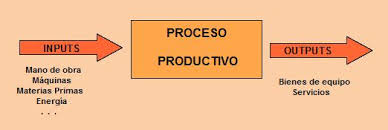
\includegraphics[scale=.4]{Proceso.jpeg}
\end {center}

\begin{itemize}
\item La tierra (o recursos naturales): todo lo que aporta la naturaleza al proceso productivo.
\item El trabajo: el tiempo y las capacidades intelectuales dedicadas a las actividades productivas.
\item El capital: los bienes duraderos no dedicados al consumo sino a producir otros bienes (máquinas y edificios).
\end{itemize}

\item \textbf{¿Que papel tiene la iniciativa empresarial en la produccion?}
\\
\textbf{Rta:}Los empresarios o las unidades económicas de producción denominadas empresas son importantes ya que nos proveen los bienes y servicios, a través de la combinación de los inputs para crear los outputs, destinados al consumo o su uso en la producción.


\item \textbf{¿Cuales son los problemas economicos a los que se enfrenta toda sociedad?}
\\
\textbf{Rta:} Como hemos señalado, el hecho de que los factores productivos estén disponibles en cantidades limitadas y que las necesidades humanas sean prácticamente ilimitadas plantea la inevitabilidad de la elección.
\begin{itemize}
\item ¿Qué producir?
\item ¿Cómo producir?
\item ¿Para quién producir?
\end{itemize}


	

\item \textbf{¿Que explica la forntera de posibilidades de produccion?}
\\
\textbf{Rta:}La frontera de posibilidades de producción muestra el máximo de combinaciones de productos que la economía puede producir utilizando todos los recursos con los que cuenta, y manifiesta la disyuntiva existente en el sentido de que una mayor cantidad producida de un bien supone una disminución de otro.
\begin {center}
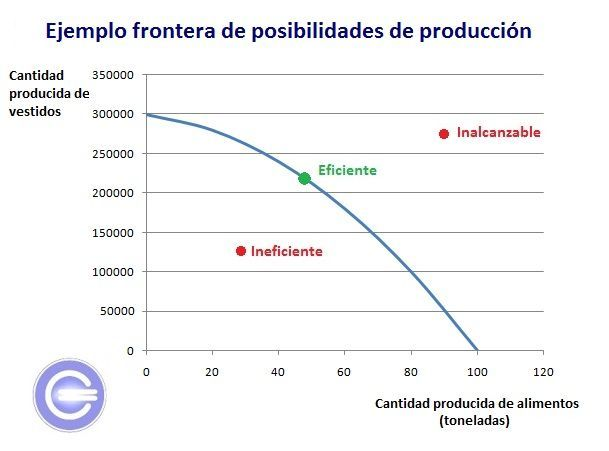
\includegraphics[scale=.4]{FPP.jpeg}
\end {center}

\item \textbf{¿Como es el costo de oportunidad a medida que se producen mas unidad de un bien?}
\\
\textbf{Rta:}El costo de oportunidad de una cosa es aquello alo que se renuncia para
conseguirla.
Si estamos obteniendo una combinación determinada de bienes empleando eficazmente todos los recursos de que dispone la sociedad, y quisiéramos producir algunas unidades más de uno de los bienes, esto tendrá que hacerse a costa de reducir la producción de otro. Esta elección entre los dos bienes indica que el costo de obtener más unidades de uno es precisamente dejar de producir algunas unidades del otro.



\item \textbf{¿Que ventajas ofrece la especializacion?}
\\
\textbf{Rta:} Para determinar qué producir y cómo producir de una forma eficiente, todas las sociedades emplean el intercambio, ya que este permite la especialización.
La especialización tiene lugar cuando los individuos y los países concentran sus esfuerzos en un conjunto particular de tareas. Esto permite que utilicen sus capacidades y recursos de la mejor manera posible.
La especialización permite reducir los costos y, a su vez, que los consumidores obtengan los productos a un precio más bajo;


\item \textbf{¿Porque surgen fallas en los mercados?}
\\
\textbf{Rta:}Rta: Una falla de mercado tiene lugar cuando un mercado no asigna eficientemente los recursos por sí mismo.
Las razones principales por las que pueden surgir fallas de mercado son las siguientes:
\begin{itemize}
\item Competencia imperfecta.
\item Externalidades
\item Información imperfecta.

\end{itemize}
.

\item \textbf{¿Que ventajas tiene la utilizacion de la clausula “Ceteris paribus”?}
\\
\textbf{Rta:} Esta condición consiste en suponer que si, por ejemplo, estamos estudiando la
incidencia del precio de los automóviles en la cantidad demandada de este bien, las demás variables que inciden en la demanda de automóviles, excepto el precio,
permanecen constantes.
La clausula nos permite  realizar experimentos controlados con los agentes económicos.


\item \textbf{¿Que se entiende por eficiencia?}
\\
\textbf{Rta:} La eficiencia es una propiedad según la cual la sociedad aprovecha de la mejor manera posible sus recursos escasos.
Cuando una economía esta situada sobre sus fronteras de posibilidades de producción es eficiente, los que se encuentran por debajo de la misma son ineficientes y los que están más allá de ella se representa como lo inalcanzable, pues la sociedad no tiene suficientes recursos para producir esa combinación de bienes.

\end{enumerate}

\chapter{EJERCICIOS Y APLICACIONES}
\section{Ejercicioss}
\begin{enumerate}
\item \textbf{Es cierto que cuando se introduce una mejora tecnológica en la producción de un bien, después del cambio hacen falta cantidades menores de recursos para generar la misma cantidad de ese bien.}
\\
Efectivamente, un desplazamiento hacia fuera de la curva de posibilidades de producción se puede lograr, por ejemplo, a través de una innovación tecnológica que permita obtener, con los recursos existentes, un aumento en la capacidad productiva de la economía. Dicho en otras palabras se puede obtener mas productos con los mismos recursos o los mismos productos son menos recursos.

\item \textbf{Comente la siguiente afirmación: Cuando disminuye el desempleo en un país, la frontera de posibilidades de producción se desplaza hacia la derecha.}
\\
Es correcta ya que, el crecimiento económico puede tener lugar por ejemplo por Aumento de la fuerza de trabajo, supone el aumento
de la capacidad productiva de la economía. Gráficamente, se puede representar mediante un desplazamiento hacia la derecha de la FPP.

\item \textbf{Considerando la frontera de posibilidades de producción entre cañones y manteca, se observa que, cuando mejora la tecnología aplicada en la producción de manteca, la frontera se desplaza de tal manera que permite producir no solo más cantidad
de este bien, sino también mayor cantidad de cañones para la misma cantidad de manteca. ¿Cómo se puede explicar este hecho?}
\\
La tecnología aplicada en la producción de manteca tambien es usada en la produccion de cañones.

\item \textbf{Analice las características del método científico que utiliza la Economía y comente los elementos que hacen que la Economía se diferencie de las demás ciencias sociales.}
\\
Las teorías no deben evaluarse por el realismo de sus supuestos sino por la validez de sus predicciones.
Al igual que la Medicina, que tiene que investigar para poder avanzar en el tratamiento de las enfermedades, la Economía, para poder profundizar en el conocimiento de la realidad y en la formulación de teorías explicativas, también necesita investigar.

lo que ocurre es que son más visibles, pues se trata de una ciencia social, y los problemas debatidos preocupan al pueblo en general. Esto no sucede en otras disciplinas, ya que quedan reducidos a la comunidad científica.

\item \textbf{Analice las siguientes afirmaciones y señale cuáles corresponderían a la Economía positiva y cuáles a la Economía normativa.}
\begin{enumerate}
\item Un incremento de los salarios generará un incremento del consumo. \textbf{Economía positiva}
\item El Estado debe garantizar la asistencia sanitaria a toda la sociedad.\textbf{Economía normativa}
\item Es conveniente reducir los impuestos para que aumente el consumo de las familias.\textbf{Economía normativa}
\item Si aumenta el precio de la vivienda, los constructores tendrán más incentivos para seguir edificando.\textbf{Economía positiva}
\end{enumerate}



\end{enumerate}

\chapter{Conclusiones}
La econom\'ia es una ciencia ya que tiene un metodo cientifico, y es social, porque el objeto de estudio es la sociedad, esta abierto el debate respecto a la economia positiva versus la economia normativa, semejante al debate que existe entre el iuspositivismo y el iusnaturalismo, ambas corrientes tienen seguidores y detractores, pero parece que la mirada positiva se va imponiendo.
\end{document}
